\documentclass{article}
\usepackage[utf8]{inputenc}
\usepackage{amsmath}
\usepackage{graphicx}
\usepackage{tikz}
\usepackage{amssymb}
\usepackage{listings} % for the source code
\usepackage{xcolor} % for the source code as well

% basic options for putting the source code
\definecolor{codegreen}{rgb}{0,0.6,0} 
\definecolor{codegray}{rgb}{0.5,0.5,0.5} \definecolor{codepurple}{rgb}{0.58,0,0.82} \definecolor{backcolour}{rgb}{0.95,0.95,0.92} 
\lstdefinestyle{mystyle}{ 
    backgroundcolor=\color{backcolour}, 
    commentstyle=\color{codegreen}, 
    keywordstyle=\color{magenta}, 
    numberstyle=\tiny\color{codegray}, 
    stringstyle=\color{codepurple}, 
    basicstyle=\ttfamily\footnotesize, 
    breakatwhitespace=false, 
    breaklines=true, 
    captionpos=b, 
    keepspaces=true, 
    numbers=left, 
    numbersep=5pt, 
    showspaces=false, 
    showstringspaces=false, 
    showtabs=false, 
    tabsize=2 } 
\lstset{style=mystyle}



\title{STAT387 HOMEWORK$\#$1 \linebreak \linebreak
\large INTRODUCTION TO STATISTICAL LEARNING}
\author{Saeah Go}
\date{Due January 14, 12:00PM}

\begin{document}

\maketitle

\section*{\underline{Conceptual}}

\subsection*{1. 2(a, b, and c)}
2. Explain whether each scenario is a classification or regression problem, and indicate whether we are most interested in inference or prediction. Finally, provide $n$ and $p$. \\
(a) We collect a set of data on the top $500$ firms in the US. For each firm we record profit, number of employees, industry and the CEO salary. We are interested in understanding which factors affect CEO salary. \\
\indent\indent This scenario is a \textbf{regression} problem, since the response (the CEO salary) is quantitative(continuous). And we are most interested in \textbf{inference} because we would like to figure out the relations how predictors affect CEO salary, not predicting something. $n$, the number of observations is $500$, and $p$, the number of predictors is $3$ (profit, number of employees, and industry) \\
(b) We are considering launching a new product and wish to know whether it will be a success or a failure. We collect data on 20 similar products that were previously launched. For each product we have recorded whether it was a success or failure, price charged for the product, marketing budget, competition price, and ten other variables. \\
\indent\indent In this scenario, we want to make sure a new launching product will be a success or failure. Since the response is a binary value (success or failure), it is categorical, thus this is a \textbf{classification} problem. Since we want to predict a result about products, we are most interested in \textbf{prediction}. In this case, $n$ is $20$ and $p$ is 13 (price charged for the product, marketing budget, competition price, and ten other variables). \\
(c) We are interesting in predicting the \% change in the US dollar in relation to the weekly changes in the world stock markets. Hence we collect weekly data for all of 2012. For each week we record the \% change in the dollar, the \% change in the US market, the \% change in the British market, and the \% change in the German market. \\
\indent\indent The scenario (c) is a \textbf{regression} problem, since the response (the \% change in the US dollar in relation to the weekly changes in the world stock markets) is quantitative(continuous) values. And in this scenario, we are interested in predicting the response, thus this is a \textbf{prediction} problem. $n$ in this case is $52$, and $p$ is 3 (the \% change in the US market, the \% change in the British market, the \% change in the German market).

\subsection*{2. 4(a and b)}
You will now think of some real-life applications for statistical learning. \\
(a) Describe three real-life applications in which classification might be useful. Describe the response, as well as the predictors. Is the goal of each application inference or prediction? Explain your answer. \\
\indent\indent 1. Stock price: Classify whether a stock will go up or down in price the next day given a set of financial data \& news from the preceding week. The aim is to make a prediction. The response would be stock market result, (go up or down), and the predictors can be the dividend–price ratio, the earnings growth rate, and the price–earnings ratio growth rate, etc. \\
\indent\indent 2. House value: Consider a real estate setting where one would like to relate values of homes to variables such as quality of schools, crime rates, closeness to a park. Say we are interested in predicting the value of a house given its characteristics. Since we want to predict a house value, the aim is to make a prediction. The response is values of homes, and the predictors are quality of schools, crime rates, and closeness to a park. \\
\indent\indent 3. Weather: Say we want to see if Portland will be rain or not tomorrow. We are interested in the thing that it will rain or not, so our goal is to make a prediction. The response will be the result (rain or not), and the predictors can be the atmospheric temperature (if temperature is below 32, it's possible to have snow rather than rain), wind speed, wind direction, amount of clouds (no clouds, then probably no rain!). \\
\linebreak (b) Describe three real-life applications in which regression might be useful. Describe the response, as well as the predictors. Is the goal of each application inference or prediction? Explain your answer. \\
\indent\indent 1. Advertising data: Consists of sales of particular product in 200 different markets, together with advertising budgets for the product in TV, radio, and newspaper. The goal is to figure out how to allocate the advertising budgets in the three media. The response would be the sales, and the predictors will be budgets for TV, radio, and newspaper. Since Y (sales) is continuous values, regression might be useful for this problem. The goal of this application is inference since we want to see the relationship between Y and X. \\
\indent\indent 2. House value: Consider a real estate setting where one would like to relate values of homes to variables such as quality of schools, crime rates, closeness to a park. Let's say we are interested in how the predictors affect the price of the house. We want to understand the relationship between the Y (house value) and the X (the elements we assumed these might affect house values), thus inference is the goal. The response is values of homes, and the predictors are quality of schools, crime rates, closeness to parks. \\
\indent\indent 3. Salary: Let's say I am thinking of changing jobs (companies). And say I got a job offer and want to see if the offered salary is higher, lower, or about to average. This case our goal is inference because we want to look how the predictors affect the salary. The response is salary, and the predictors are years of experience, education level, industry, location (big city, suburban or rural area).

\section*{\underline{Applied}}
\subsection*{3. 9(a, b, c, d, e, f)}
This exercise involves the Auto data set studied in the lab. Make sure that the missing values have been removed from the data. \\
\linebreak (a) Which of the predictors are quantitative, and which are qualitative? \\
\indent\indent Quantitative Variables are the variables whose values result from counting or measuring something. (Continuous) Qualitative Variables are the variables that are not measurement variables. (Categorical) Their values do not result from measuring or counting. \\
Thus, the quantitative predictors are: mpg, displacement, horsepower, weight, and acceleration. \\
And, the qualitative predictors are: cylinders, year, origin, and name. \\
\linebreak (b) What is the range of each quantitative predictor? You can answer this using the range() function. \\
\indent\indent I used R to answer this question. 
\begin{center}
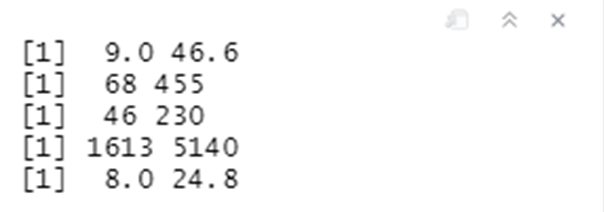
\includegraphics[scale = 0.46]{3.9.b.png} \\
\end{center}
The range of mpg is $46.6 - 9.0 = 37.6$ \\
%The range of cylinders is: $8 - 3 = 5$ \\
The range of displacement is: $455 - 68 = 387$ \\ 
The range of horsepower is: $230 - 46 = 184$ \\
The range of weight is: $5140 - 1613 = 3527$ \\
The range of acceleration is: $24.8 - 8.0 = 16.8$ \\
\linebreak (c) What is the mean and standard deviation of each quantitative predictor? \\
\indent\indent I also used R to answer this question. I rounded to the nearest 0.01. \\
\begin{center}
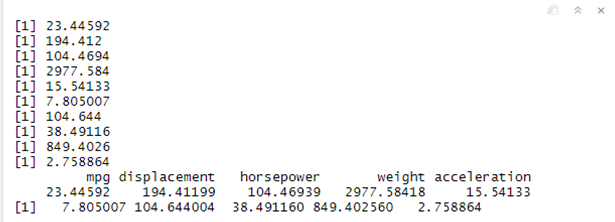
\includegraphics[scale = 0.46]{3.9.c.png} \\
\end{center}
The mean of mpg is: 23.45 \\
%The mean of cylinders is: 5.47 \\
The mean of displacement is: 194.41 \\
The mean of horsepower is: 104.47 \\
The mean of weight is: 2977.58 \\
The mean of acceleration is: 15.54 \\
%The mean of year is: 75.98 \\
\linebreak The standard deviation of mpg is: 7.81 \\
%The standard deviation of cylinders is: 1.71 \\
The standard deviation of displacement is: 104.64 \\
The standard deviation of horsepower is: 38.49 \\
The standard deviation of weight is: 849.40 \\
The standard deviation of acceleration is: 2.76 \\
%The standard deviation of year is: 3.68 \\
\linebreak (d) Now remove the 10th through 85th observations. What is the range, mean, and standard deviation of each predictor in the subset of the data that remains? \\
\indent\indent I used R for this question again. \\
\begin{center}
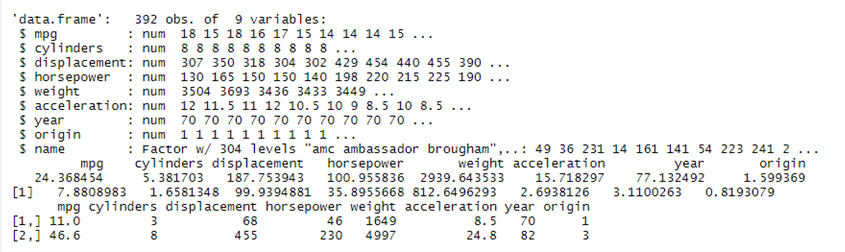
\includegraphics[scale = 0.46]{3.9.d.png} \\
\end{center}
The range of mpg is $46.6 - 11.0 = 35.6$ \\
The range of cylinders is: $8 - 3 = 5$ \\
The range of displacement is: $455 - 68 = 387$ \\ 
The range of horsepower is: $230 - 46 = 184$ \\
The range of weight is: $4997 - 1649 = 3348$ \\
The range of acceleration is: $24.8 - 8.5 = 16.3$ \\
The range of year is: $82 - 70 = 12$ \\
The range of origin is: $3 - 1 = 2$ \\
\linebreak The mean of mpg is: $24.37$\\
The mean of cylinders is: $5.38$ \\
The mean of displacement is: $187.75$ \\
The mean of horsepower is: $100.96$ \\
The mean of weight is: $2939.64$ \\
The mean of acceleration is: $15.72$ \\
The mean of year is: $77.13$ \\
The mean of origin is: $1.60$ \\
\linebreak The standard deviation of mpg is: $7.88$ \\
The standard deviation of cylinders is: $1.66$ \\
The standard deviation of displacement is: $99.93$ \\
The standard deviation of horsepower is: $35.90$ \\
The standard deviation of weight is: $812.65$ \\
The standard deviation of acceleration is: $2.69$ \\
The standard deviation of year is: $3.11$ \\
The standard deviation of origin is: $0.82$ \\
\linebreak (e) Using the full data set, investigate the predictors graphically, using scatter plots or other tools of your choice. Create some plots highlighting the relationships among the predictors. Comment on your findings. \\
\indent\indent I used R to create some plots. \\
\underline{Plots} 
\begin{center}
    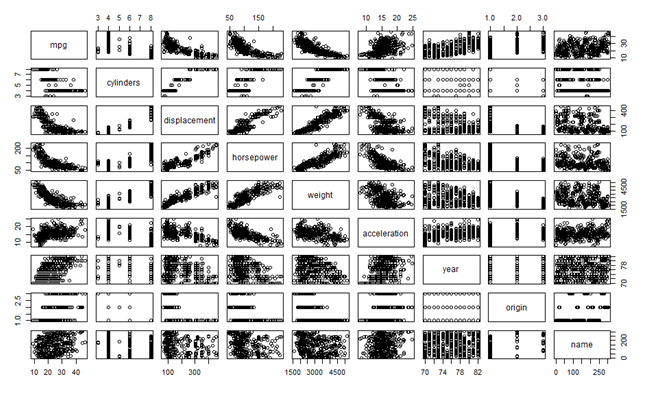
\includegraphics[scale = 0.6]{3.9.e-2.png} 
    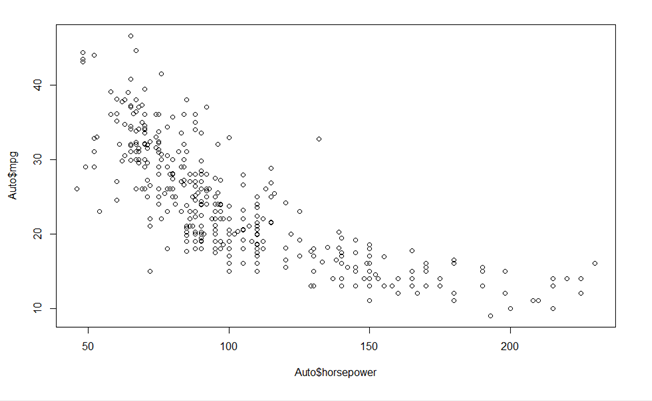
\includegraphics[scale = 0.6]{3.9.e-3.png} 
    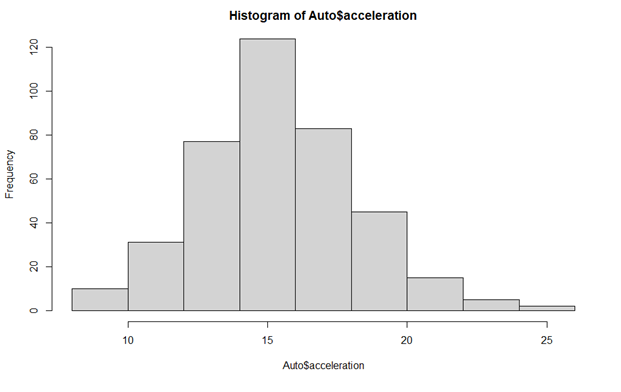
\includegraphics[scale = 0.6]{3.9.e-4.png} 
\end{center}
\underline{My findings} 
\linebreak 
\indent * The histogram for `acceleration' resembles a normal distribution. \\
\indent * From the pairs(Auto), I could find that `displacement' and `weight' have a strong linear relationship. \\
\indent  * `mpg' has a non-linear relationship with `displacement', `horsepower', and `weight'. \\
\linebreak (f) Suppose that we wish to predict gas mileage (mpg) on the basis of the other variables. Do your plots suggest that any of the other variables might be useful in predicting mpg? Justify your answer. \\
\indent\indent Yes. My plots suggest that year, horsepower, weight, and displacement might be useful in predicting mpg. I noticed these variables have positive or negative relationships to the mpg outcome. For example, I could notice that year and mpg have a positive relationship (As the year increases, the mpg also tends to increase). Also I could find that horsepower and mpg appear to have a negative relationship (As the horsepower increases, the mpg tends to decrease). Similarly, weight and mpg, have a negative relationship too. (As the weight of car increases, the mpg tends to decrease). Displacement and mpg also have a negative relationship. (As the displacement increases, the mpg tends to decrease). 


\section*{\underline{R Code}}
\begin{lstlisting}[language=R]
# Applied
## 3. 9 (a, b, c, d, e, f)

#################################################
### Problem (a)
#################################################
data(Auto, package = "ISLR") # load the data
fix(Auto) # since I already have loaded the ISLR package with the "library" command, I don't need to use "read.table" command to load the "Auto" data. It is already loaded in R. I can view the file using the command "fix(Auto)".


#################################################
### Problem (b)
#################################################
range(Auto$mpg)
range(Auto$displacement)
range(Auto$horsepower)
range(Auto$weight)
range(Auto$acceleration)


##################################################
### Problem (c)
##################################################
# Method 1 (simply use mean() and sd() functions)
mean(Auto$mpg)
mean(Auto$displacement)
mean(Auto$horsepower)
mean(Auto$weight)
mean(Auto$acceleration)

sd(Auto$mpg)
sd(Auto$displacement)
sd(Auto$horsepower)
sd(Auto$weight)
sd(Auto$acceleration)

# Method 2 (use colMeans() and colSds())
colMeans(Auto[,c(1, 3:6)])
colSds(as.matrix(Auto[,c(1, 3:6)])) # need to make the data to matrix form

###################################################
### Problem (d)
###################################################
# drop rows using slice() function in the dplyr package
new_Auto <- Auto %>% slice(-c(10:84)) # remove from 10th to 85th observations

# check the structure of the Auto dataset
str(Auto) # since name's structure is factor (not numeric values), I cannot get mean and standard deviation with the name column.

# find means and standard deviations of only numeric columns (except name)
colMeans(new_Auto[,c(1:8)])
colSds(as.matrix(new_Auto[,c(1:8)]))
sapply(new_Auto[, c(1:8)], range)


###################################################
### Problem (e)
###################################################
pairs(Auto) # method 1
pairs(~ mpg + cylinders + displacement + horsepower + weight + acceleration + year + origin + name, Auto) # method 2

plot(Auto$horsepower, Auto$mpg)
hist(Auto$acceleration)
\end{lstlisting}


\end{document}